\chapter{Background} \label{cha:background}

In this chapter, we will introduce Magnolia in section \ref{sec:magnolia}, some
of the interesting aspects the language introduces, and examples of how we can
use it. We will then discuss \gls*{ide}s in the following section \ref{sec:ide},
and mention some specific functionality they have that make them great tools for
developers. Then, in section \ref{sec:architecture}, we will cover our
approach, and how it differs from standard modularity in other \gls*{ide}s. We
will also address the current Magnolia \gls*{ide}. Finally, in the last section
\ref{sec:challenges} we will discuss the challenges that exist due to the
uniqueness of the Magnolia language.


\section{Magnolia} \label{sec:magnolia}

Magnolia is designed to support a high level of abstraction and ease of
reasoning. It was created with the purpose of being highly extensible,
allowing for experimentation of language features, like functionalization,
mutification, generated types and type partitions. With
Bagge~\cite{baggeThesis}, we can summarize a Magnolia program to three
fundamental ideas.

\begin{itemize}
  \item \textit{Concept}: A set of operations, type declarations and axioms.
  \item \textit{Implementation}: Implementation of a concept.
  \item \textit{Satisfaction}: Satisfaction of an implementation.
\end{itemize}

While Magnolia is inspired by things like abstract algebra and institution
theory, it is quite trivial to understand on a conceptual level. Developers quite
often work with sets of operations, type declarations and axioms, namely
\gls*{api}s.

\subsection{Magnolia concept}

Commonly, the term \gls*{api} is used specifically for \gls*{rest} \gls*{api}s, but
it also covers concepts, like those in Magnolia, interfaces in Java, traits in
Rust, or type-classes in Haskell. What all of these variations have in common,
is that they specify a method for two different procedures to communicate with
each other. In a \gls*{rest} \gls*{api} this could be a microservice architecture,
where several servers send and receive requests and responses, or in a
programming project, it could be the \textbf{List} interface in Java, which
informs consumers of that interface, which methods are needed to qualify as a
\textbf{List}. In Magnolia a concept declare types, functions and properties
which those functions need to uphold. A simple example of this would be a
concept for addition with natural numbers.

\begin{center}
  \lstinputlisting
    [ language=Magnolia
    , caption={Natural numbers (Magnolia)}
    , label=lst:nat
    ]{./code/magnolia-nat.mg}
\end{center}

In the listing \ref{lst:nat}, we are specifying concept called
\textit{NaturalNumbers}, which declares a type \textbf{N}, and three methods
that act upon the type \textbf{N}. We have the function\footnote{Also called a constructor}
\textbf{zero}, which takes zero arguments, and should return something of type
\textbf{N}. With this constructor, we can instantiate our numbers. To get new
numbers, we have the function \textbf{succ}, which should give the
\textit{succ}essor to the passed number. That way, we can represent $0$ as
\textbf{zero()}, $1$ as \textbf{succ(zero())}, and $2$ as
\textbf{succ(succ(zero()))}. The final function, is an infix operator. $+$ takes
two arguments of type \textbf{N} and returns an \textbf{N}. Of course, this
should be interpreted as addition, meaning \textbf{succ(zero())} $+$
\textbf{succ(succ(zero()))} $=$ \textbf{succ(succ(succ(zero())))}, or using
numbers: $1 + 2 = 3$. Finally, the last statement in the concept is an axiom,
stating that given any $a$, if we add \textbf{zero()} to $a$, we should get $a$,
of type \textbf{N}.

This axiom is what allows for us to put constraints on our concepts, which
allows for improvement in our \gls*{api}. Unlike other \gls*{api}s, like traits or
\gls*{rest}, such specific constraints can only be achieved by using unit tests,
which is not enforced on the implementor. But with axioms, this is possible in
Magnolia. This pattern is quite useful, since it allows for \textit{reuse} of
logic. The listings \ref{lst:list} specifies a list interface, we can
instantiate a list, and do operations on it, such as getting adding an element to
the list, or by concatenating two lists. We can also fetch the first element of
the list, by using \textbf{head}, note the \textit{guard} attached to the
function statement, this guard ensures that when this method is invoked, the
list we get the first element from, cannot be empty\footnote{Meaning it is equal to \textbf{nil()}},
which means that our function is not \textit{total}, but \textit{partial}. This
means that for any argument, we might not have a corresponding result. If we did
not have this guard, then what would happen if we \textit{took} \textbf{head} of a list
with no elements? In languages like Java, we would get null, but this does not
exist in Magnolia. We could expand upon the list \gls*{api} by creating a
non-empty variant of list, as shown in listing \ref{lst:nonList}, which is the
same as list, except to instantiate it, we need to supply an element, ensuring
when we have a \textbf{NonEmptyList} variant, we can safely get an element from
it, since there will at minimum be one element in the list, due to our
constructor requiring one argument.

\begin{code}[H]
  \lstinputlisting
    [ language=Magnolia
    , caption={List concept (Magnolia)}
    , label=lst:list
    ]{./code/magnolia-list.mg}
\end{code}

\begin{code}[H]
  \lstinputlisting
    [ language=Magnolia
    , caption={NonEmptyList concept (Magnolia)}
    , label=lst:nonList
    ]{./code/magnolia-non-list.mg}
\end{code}

However, the interpretation we have assigned to the \textit{NaturalNumbers},
\textit{List}, and \textit{NonEmptyList} concept, depends on our implementation.

\subsection{Magnolia implementation}

As one can see in listing \ref{lst:impl}, we have implemented the concept
specified in listing \ref{lst:nat}, by using concrete values for \textbf{N}.
There is an implementation for all the functions, giving us the functionality we
set out to specify with our concept, but there is nothing stopping us from
straying away from the specification, by implementing it incorrectly. Since we
are using primitive types\footnote{In this case, integers, specifically 32-bit}
we have to use external code, which is another feature of Magnolia. In the\
listings \ref{lst:impl} and \ref{lst:impl-wrong}, we are using an external
implementation of numbers, from C++.

\begin{code}[H]
  \lstinputlisting
    [ language=Magnolia
    , caption={Natural numbers implementation (Magnolia)}
    , label=lst:impl
    ]{./code/magnolia-add.mg}
\end{code}

\begin{code}[H]
  \lstinputlisting
    [ language=Magnolia
    , caption={Invalid implementation (Magnolia)}
    , label=lst:impl-wrong
    ]{./code/magnolia-add-wrong.mg}
\end{code}

We have defined the function \textbf{zero} correctly in listing
\ref{lst:implCpp}. On line five, we return $0$, which is what we expect, based
on our axiom. However, on line 5, in listing \ref{lst:implCppWrong}, we instead
return $1$, which breaks our axiom, as $1 + 1 \neq 1$.

\begin{code}[H]
  \lstinputlisting
    [ language=C++
    , caption={Natural numbers implementation (C++)}
    , label=lst:implCpp
    , numbers=left
    , numberstyle=\tiny\color{gray}
    ]{./code/CxxNaturalNumbers.hxx}
\end{code}

\begin{code}[H]
  \lstinputlisting
    [ language=C++
    , caption={Invalid implementation (C++)}
    , label=lst:implCppWrong
    , numbers=left
    , numberstyle=\tiny\color{gray}
    ]{./code/CxxNaturalNumbersWrong.hxx}
\end{code}

This is where the
\textit{satisfaction} comes in, it is what ties the concept and implementation
together, by ensuring our axiom are upheld.

\subsection{Magnolia satisfaction}

\begin{center}
  \lstinputlisting
    [ language=Magnolia
    , caption={Satisfaction of the natural numbers (Magnolia)}
    , label=lst:sat
    ]{./code/magnolia-sat.mg}
\end{center}

When implementing a concept in Magnolia, one could do so incorrectly. In other
programming languages, one might still have \textit{imparted} some meaning in an
interface, like that in Java, the interface \textbf{List} in the standard
library, the method \textbf{addAll} is an associative operation, as shown in
the following listing, \ref{lst:listConcat}, where we expect the assertion to be
true.

\begin{code}
  \lstinputlisting
    [ language=Java
    , caption={List concatenation that should result in the same list. (Java)}
    , label=lst:listConcat
    ]{./code/list-concat.java}
\end{code}

Of course, this is the case in the standard library to Java, but there is
nothing that enforces this property on other implementers of the interface.
Usually, programmers who want such a property on their interfaces, create unit
tests, testing that it is the case that \textbf{addAll} is associative. But to
enforce this, one would have to create a unit test for each implementation of
the interface, while in Magnolia one writes a satisfaction as shown in listing
\ref{lst:sat}, which in turn is \textit{transpiled} to a format understandable
by an \gls*{smt} solver. This \gls*{smt} solver can \textit{prove} that our
implementation upholds our axioms in the implemented concept. Importantly, this
can be done for any consumer of the \gls*{api}.


\subsubsection{Satisfiability Modulo Theories solvers}

A \gls*{smt} solvers are programs that \textit{prove} first-order formulas.
Skogvik~\cite{beateVerification} showcases how Magnolia concepts can be
translated into such first-order formulas, and be used by \gls*{smt} solvers to
verify them. Skogvik also lays out different \gls*{smt} solvers and compare them
against each other, with the Magnolia library as input. One of Skogviks
conclusions are that while verification of some program is good to have, some
features needed for a new \gls*{ide} would be to integrate it with this
functionality.


\subsection{Mathematics and programming}

Mathematics is everywhere, and useful. It's not always easy to notice this, but
one thing that helps, is knowing the names of the structures one encounter. One
can easily understand that knowing simple operations like addition,
multiplication, etc.\ is useful but for more abstract mathematics, this is
harder. An example of this is abstract algebra, which is the study of algebraic
structures, which are often seen in programming. A programmer will use these
structures more often than not, knowingly or unknowingly, and a good programmer
will explicitly seek these structures out.

An important aspect of development, is logging. Knowing what actions have taken
place is an essential tool when hunting down bugs. A common way to structure
logs, would be composing them depending on when in the call stack they occurred.
As a concrete example, let's say we are making a text editor, and are in the
need of a logging manager, which, among other things, should compose different
log statements. Assuming we have some type \textbf{Log(A)}, where the type
\textbf{A}, is the result of the computation of a given function, we want to be
able to compose different, related, computations. But, importantly, the order of
composition of the \textbf{Log(A)}-type matters. Representing the composition of
the \textbf{Log(A)}-type as $\odot$, and letting $a, b, c$ be of type
\textbf{Log A}:

\begin{definition}[Log Composition] \label{def:logComp}
  \begin{equation}
    a \odot \left ( b \odot c \right ) = \left ( a \odot b \right ) \odot c
  \end{equation}
\end{definition}

Now we have a good logger, as the logs of the entire call stack is available for
us to read when something goes wrong. Moving on, a good feature of a text
editor, is being able to undo and redo actions. These are the actions that a
user should be able to do:

\begin{itemize}
  \item Insert text at a position
  \item Delete text from a position
  \item Redo an action
  \item Undo an action
\end{itemize}

Same as in the logging example, composing is a reasonable thing to implement,
and should result in another action. Similarly, the order matters; deleting text
and then inserting, is not the same as inserting and then deleting. But what is
different between the logging and editor example, is that we also want the
\textit{inverse} of an action, so for every action we want an opposite action
that undos an action. Say, $a$ is some action, and $b$ is some opposite action,
then our composition looks like this:

\begin{definition}[Action Composition] \label{def:actComp}
  \begin{equation}
    a \odot b = U
  \end{equation}
\end{definition}

Where $U$ is an action representing \textit{no-operation}. This could be
inserting the empty string at any position, deleting the empty string at any
position, or redoing or undoing any of the aforementioned actions.

Both of these examples are relatively easy to implement, but harder to verify,
to ensure they satisfy our properties; that the \textit{logic} holds. In Java
and Rust, to ensure that we have implemented something correctly, one would
create a unit test. But there is nothing to ensure that we create this test
correctly, that we cover all the edge cases, or if we are testing the correct
thing.

\subsection{Logging example in Java, Rust, and Magnolia}

In the Java listing (\ref{lst:jlogging}) and Rust listing (\ref{lst:rlogging})
we have implementations of logging which might not uphold our constraints. We
can add unit tests, that ensure the implementations satisfy the definition
\ref{def:logComp}, but this safeguard only exists in our project, and once our
\gls*{api} can be implemented by third-party developers, we have no guarantee
they will follow our constraints.

\begin{center}
  \lstinputlisting
    [ language=Java
    , caption={Logging structure (Java)}
    , label=lst:jlogging]{./code/logging.java}
\end{center}

\begin{center}
  \lstinputlisting
    [ language=Rust
    , caption={Logging structure (Rust)}
    , label=lst:rlogging]{./code/logging.rs}
\end{center}

In Magnolia, however, it is possible to constrain a consumer of our \gls*{api}.
In the listing \ref{lst:mlogging}, we can add an axiom, which is the same as our
requirement definition \ref{def:actComp}. For implementers, \textit{consumers}
of our \gls*{api}, we can now ensure they implement correctly, as long as they
add the simple declaration showed in listing \ref{lst:mlogSat}. This will be
ensured, because in a standard Magnolia work routine, a developer will invoke an
\gls*{smt} solver, which will ensure the concepts, that are implemented are
sound; that they are satisfiable.

\begin{center}
  \lstinputlisting
    [ language=Magnolia
    , caption={Logging structure (Magnolia)}
    , label=lst:mlogging]{./code/logging.mg}
\end{center}

\begin{center}
  \lstinputlisting
    [ language=Magnolia
    , caption={
        Magnolia logging satisfaction, the implementation is left out for
        brevity
      }
    , label=lst:mlogSat]{./code/logging-sat.mg}
\end{center}

\subsection{Editor example in Java, Rust, and Magnolia}

The Java and Rust listings, (\ref{lst:jeditor}, \ref{lst:reditor}), also have no
method of ensuring the satisfiability of future implementations. But what is
more interesting, is that we can see, clearily in the case of the Magnolia
listing \ref{lst:meditor}, that there is some kind of relation between these
\gls*{api}s.

\begin{code}[H]
  \lstinputlisting
    [ language=Java
    , caption={Editor structure (Java)}
    , label=lst:jeditor]{./code/editor.java}
\end{code}

\begin{code}[H]
  \lstinputlisting
    [ language=Rust
    , caption={Editor structure (Rust)}
    , label=lst:reditor]{./code/editor.rs}
\end{code}

\begin{code}[H]
  \lstinputlisting
    [ language=Magnolia
    , caption={Editor structure (Magnolia)}
    , label=lst:meditor]{./code/editor.mg}
\end{code}

Both the logging example, and the text editor example, are some binary operation\footnote{Function with two arguments}
over some set. In the first example, our set was all different log statements of
the type \textbf{Log A}, and composing these logs, gave us another
\textbf{Log A} type. While in the second example, we were working on the set of
actions, which we could compose, which also gave us another action, but we also
had an action representing no-operation, and an \textit{inverse} operation,
undoing an action. This is related to mathematics, specifically abstract
algebra, the study of algebraic structures.

\subsection{Abstract algebra}

In the first example, we are working with a \textit{semigroup}, and in the
second example, we are working with a \textit{group}. These are known as
algebraic structures, which is just some set, with a function that takes two
inputs, and outputs one result, and some property on that function. The trivial
example, is known as \textit{magma}, and is defined in \ref{def:magma}. The
closure definition \ref{def:closed} simply specifies that we only work with one
set.

\begin{definition}[Closure] \label{def:closed}
  For a set $M$, with a binary operation $\oplus$,
  $\forall a, \forall b, \exists c \in M$, such that
  $a \oplus b = c$.
\end{definition}

\paragraph{Closure} Addition with the integers is a kind of closure, as per the
definition \ref{def:closed}, since no matter what integer you put into the
equation, you will still get an integer. And since this is the only requirement a
magma has, this example is also a magma.

\begin{definition}[Magma] \label{def:magma}
  A magma is a set $M$, with a binary operation $\oplus$, which is
  \textit{closed} by definition \ref{def:closed}
\end{definition}

We can \textit{extend} the definition of magma, by adding associativity on the
binary operation. The definition \ref{def:assoc}, as shown in the example
\ref{exmp:assoc},
simply specifies that the order we evaluate our composition matters.

\begin{exmp} \label{exmp:assoc}
  Multiplication with the positive integers is associative, since no matter
  where we put parentheses; what order we evaluate this equation:
  $2 \times 3 \times 4$, we will get the same answer.
  $$
  (2 \times 3) \times 4 = 2 \times (3 \times 4)
  $$
\end{exmp}

\begin{definition}[Associativity Law] \label{def:assoc}
  For any binary operation $\oplus$, on a set $M$, $a, b, c \in M$.
  $a \oplus \left ( b \oplus c \right ) = \left ( a \oplus b \right ) \oplus c$,
  must hold.
\end{definition}

This associativity gives us a semigroup, as shown in the definition
\ref{def:semi}, which is the structure that we modeled in our logging example.

\begin{definition}[Semigroup] \label{def:semi}
  A semigroup is a set $M$, with a binary operation $\oplus$, and $\oplus$ must
  uphold the definitions \ref{def:closed} and \ref{def:assoc}.
\end{definition}

By simply requiring the identity law (\ref{def:ident}), we get a
monoid (\ref{def:monoid}), and adding the inverse law
(\ref{def:inv}), we get a group.

\begin{definition}[Identity Law] \label{def:ident}
  For any binary operation $\oplus$, on a set $M$, $\forall a, \exists U \in M$,
  such that $a \oplus U = a$ and $U \oplus a = a$. This makes $U$ is unique.
\end{definition}

\begin{definition}[Monoid] \label{def:monoid}
  A monoid is a set $M$, with a binary operation $\oplus$, and $\oplus$ must
  uphold the definitions \ref{def:closed}, \ref{def:assoc}, and \ref{def:ident}.
\end{definition}

\begin{exmp}
  To make a monoid, we can choose the binary operation to be $\times$, and our
  set to be the natural numbers, ($\mathbb{N}$). We know addition is closed, and
  associative, so choosing $U = 1$, we get a monoid. Any number from our set
  $\mathbb{N}$ multiplied with $1$, gives us the number we choose.
\end{exmp}

\begin{definition}[Inverse Law] \label{def:inv}
  For any binary operation $\oplus$, on a set $M$,
  $\forall a, \exists U \in M$, such that
  $a \oplus U = a$, and $U$ is unique.
  And $\forall a, \exists b \in M$, such that $a \oplus b = U$ and
  $b \oplus a = U$, and the mapping for $a \to b$ is one-to-one.
\end{definition}

\begin{definition}[Group] \label{def:group}
  A group is a set $M$, with a binary operation $\oplus$, and $\oplus$ must
  uphold the definitions \ref{def:closed}, \ref{def:assoc}, \ref{def:ident},
  and \ref{def:inv}.
\end{definition}

The definition \ref{def:group}, of course is identical to the structure we used
to model undo-redo, in our text editor example. We have our \textit{combine}
operator, which takes two variants of the \textit{action}-type, and return
another variant of the same type. It is therefore a closed binary operation. We
also specified that \textit{combine} is associative, it does not matter where one
puts the parentheses, the resulting combination of \textit{action}s are
equivalent. \textit{no-operation} gives us the \textit{unit}, meaning our binary
operation upholds the identity law. Finally, we have an inverse \textit{action}
variant, that is unique, for all other variants.

This, of course, is dependent on our implementation. It is quite common to make
mistakes when developing. These mistakes are usually tackled by developing good
unit tests. However, this can get quite tedious, as for everytime we re-implement
these algebraic structures, we would have to re-create the unit tests. To avoid
these common mistakes when implementing these structures, it would behoove a
developer if they could encode these properties in something like an interface or
a trait, however, this is not possible in either Java nor Rust. We cannot enforce
things like the definition \ref{def:assoc} on our operators.

\subsection{Java: magma to group}

This structure could \textit{technically} be implemented in something like Java
as shown in listings \ref{lst:jmagma}, \ref{lst:jsemigroup}, \ref{lst:jmonoid},
and \ref{lst:jgroup}. But not practically. Note the empty interfaces; there is
nothing that enforces the different laws; properties, on our method. This can
only be done by unit testing, which is not enforced on an external consumer of
the \gls*{api}.

\begin{center}
  \lstinputlisting
    [ language=Java
    , caption={Magma interface (Java)}
    , label=lst:jmagma]{./code/magma.java}
\end{center}

\begin{center}
  \lstinputlisting
    [ language=Java
    , caption={Semigroup interface (Java)}
    , label=lst:jsemigroup]{./code/semigroup.java}
\end{center}

\begin{center}
  \lstinputlisting
    [ language=Java
    , caption={Monoid interface (Java)}
    , label=lst:jmonoid]{./code/monoid.java}
\end{center}

\begin{center}
  \lstinputlisting
    [ language=Java
    , caption={Group interface (Java)}
    , label=lst:jgroup]{./code/group.java}
\end{center}

\subsection{Rust: magma to group}

The same issue with property enforcement exists in Rust.

\begin{center}
  \lstinputlisting
    [ language=Rust
    , caption={Magma trait (Rust)}
    , label=lst:rmagma]{./code/magma.rs}
\end{center}

\begin{center}
  \lstinputlisting
    [ language=Rust
    , caption={Semigroup trait (Rust)}
    , label=lst:rsemigroup]{./code/semigroup.rs}
\end{center}

\begin{center}
  \lstinputlisting
    [ language=Rust
    , caption={Monoid trait (Rust)}
    , label=lst:rmonoid]{./code/monoid.rs}
\end{center}

\begin{center}
  \lstinputlisting
    [ language=Rust
    , caption={Group trait (Rust)}
    , label=lst:rgroup]{./code/group.rs}
\end{center}

\subsection{Magnolia: magma to group}

However, in Magnolia this can be required on the \textit{interface}-level. The
example code shown in listing \ref{lst:magma}, showcases a concept
representation a binary operation, which has one function, \textit{binop}, which
takes in two values of type \textit{T}, and returns \textit{T}. Note that the
actual implementation of this function is missing. This is because a concept
encodes the properties of a users code. The actual implementation of the
binary function needs to uphold the properties of the concept that is
being implemented. Note that this is unlike the Java and Rust example, in
which we have no way to encode the property of our binary function. So any
consumer of our \gls*{api} would not be explicitly bound to our restriction of
the associativity law \ref{def:assoc}, identify law \ref{def:ident}, and the
inverse law \ref{def:inv}, required by semigroup and group. The closure
definition, \ref{def:closed}, however, can be encoded by the type system in Java
and Rust.

\begin{center}
  \lstinputlisting
    [ language=Magnolia
    , caption={Magma concept (Magnolia)}
    , label=lst:magma]{./code/magma.mg}
\end{center}

In the example code shown in listing \ref{lst:semigroup}, the \textit{magma}
concept has been expanded upon, still following the same rules as before, but
with the added property of associativity.

\begin{center}
  \lstinputlisting
    [ language=Magnolia
    , caption={Semigroup concept (Magnolia)}
    , label=lst:semigroup]{./code/semigroup.mg}
\end{center}

\begin{center}
  \lstinputlisting
    [ language=Magnolia
    , caption={Monoid concept (Magnolia)}
    , label=lst:monoid]{./code/monoid.mg}
\end{center}

\begin{center}
  \lstinputlisting
    [ language=Magnolia
    , caption={Group concept (Magnolia)}
    , label=lst:group]{./code/group.mg}
\end{center}

So Magnolia facilitates reuse, and extension of logic. In Magnolia we can build
upon existing proven algebraic structures like a group, and reuse their
properties. One of the interesting properties of the group structure, is that
certain evaluations are the same. In our editor example, the usefulness of this
is clearer, as we can do optimizations on the editor actions. Since the user of
the editor reacts slower than our code, we can batch several actions together,
and evaluate them together. If the user keeps writing and deleting the same
sentence over and over again, we could evaluate them as a
\textit{no-operation}, and not do the expensive operation of writing and
removing text from a file.


\subsection{Reuse in Magnolia}

One of the most important features in any programming language, is the notion
of \textit{reusability}. From the invention of the GO-TO-statement, with which
we could repeat code statements $N$ times instead of writing them $N$ times, to
functions, where we could run the same piece of code several times in a
program, with different inputs, reuse has been an essential tool for a
programmer. It avoids \textit{re-inventing the wheel}, as common functionality
can be externalized and reused in several different places. This ensures
fewer points of failure. Instead of having to test several different places in
a project, we can test the function being used different places.

Reusability is also an important feature in Magnolia, but this reusability is in
the entire language. In libraries in other languages, functions are reused, in
an attempt to avoid common logical mistakes, but these mistakes could still be
there, hiding in plain view. In Magnolia, one can re-use the \textit{logic} of a
function. The logging and group example can be rewritten using Magnolia concepts
as shown in listing \ref{lst:logging} and \ref{lst:editor} respectively, by
reusing the concepts we created for semigroup in listing \ref{lst:semigroup} and group
in listing \ref{lst:group}.

\begin{code}[H]
  \lstinputlisting
    [ language=Magnolia
    , caption={Logging example (Magnolia)}
    , numbers=left
    , numberstyle=\tiny\color{gray}
    , label=lst:logging]{./code/logging-solution.mg}
\end{code}

\begin{code}[H]
  \lstinputlisting
    [ language=Magnolia
    , caption={Editor example (Magnolia)}
    , numbers=left
    , numberstyle=\tiny\color{gray}
    , label=lst:editor]{./code/editor-solution.mg}
\end{code}

Indeed, reuse is so useful, that in Magnolia one can rename concepts one use.
In the listings \ref{lst:logging} and \ref{lst:editor}, we have renamed the type
and function into something that makes more sense in the specific use case. On
line four, in \ref{lst:logging}, we have renamed \textbf{binop} and \textbf{T}
to \textbf{combine} and \textbf{Log}, respectively.

While it is useful for us developing the concept, to know that our logging
concept is a semigroup, when using an implementation, this is less relevant.
If a consumer of the logging \gls*{api} read that logs where used everywhere in
the project with \textbf{binop(log\_a, log\_b)}, it would be confusing, but when
using context specific names, as renaming allows us to do, we could rename
\textbf{binop} to \textbf{combine}, which makes the code easier to read.


\section{Integrated Development Environment} \label{sec:ide}

Before \gls*{ide}s where the standard development tool, all a developer had, was
a terminal, an editor, and a compiler/interpreter. An editor to change the
source code, a compiler/interpreter to compile/interpret, and a terminal to
invoke them. But not all projects can be handled this way. In larger projects
other programs like
Make\footnote{\url{https://www.gnu.org/software/make/}} for C/C++, or
Gradle\footnote{\url{https://gradle.org/}} for Java/Kotlin, was needed to
build, test and package the project. So instead of manually adding each new C
file to the compiler argument list, or manually compiling and zipping Java class
files, an external program was used. But for C/C++ or Java/Kotlin, external
libraries are used, which meant that among different developers, the environment
could vary.

This meant that onboarding new developers took time, to ensure they had all the
necessary dependencies to develop the project. Which could be as simple as
downloading some library or program, to ensuring specific environment variables
existed during compile time. Eventually all of these different dependencies,
programs, environment variables and such where all integrated into a single
application.

An \gls*{ide}, aids a developer, as all the needed tools for development are
integrated into one application. Some are more specialized than others,
targeting specific language, like Eclipse and IntelliJ. Others are
more generic, like VS Code. We will use the terms generic and specialized
\gls*{ide}s to differentiate the two variants.


\subsection{Syntax highlighting}

Highlighting important keywords, identifiers and more, makes the language easier
to read for the developer, allowing them to spot easy to miss errors, like
misspelling of keywords, functions, and variables. In the pictures
\ref{pic:stx}, and \ref{pic:noStx} we can see the difference between having
syntax highlighting. In \ref{pic:stx} we can clearly see what is, and is not a
latex command, if we wrote \textit{begn} instead of \textit{begin}, we can
notice the discrepancy, as we expect it to, in this case, be purple. We are
using visualization to make developers notice issues.

\begin{figure}
  \centering
  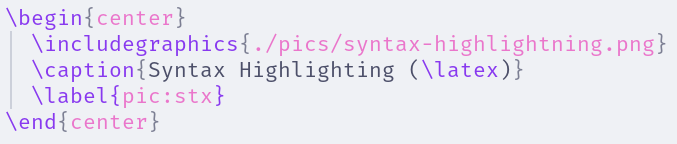
\includegraphics[width=0.5\textwidth]{syntax-highlighting.png}
  \caption{Syntax Highlighting (\LaTeX\ in Vim)}
  \label{pic:stx}
\end{figure}

\begin{figure}
  \centering
  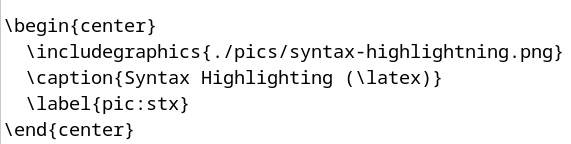
\includegraphics[width=0.5\textwidth]{no-syntax-highlighting.png}
  \caption{No Syntax Highlighting (\LaTeX\ in Vim)}
  \label{pic:noStx}
\end{figure}

\subsection{Code autocompletion}

Suggesting keywords, method names or even entire code snippets, is a powerful
tool an \gls*{ide} can have. This is possible to achieve, in some form, without
being specialized, by for example, suggesting text that already exist in the
document, but is most useful if it is specialized, and can suggest built-in
methods. This allows a developer to not having to remember exactly how methods
are named, is the method to split a string by some delimiter, \textit{split\_by}
or \textit{split\_on}? As long as the developer writes \textit{split}, the
correct method name will be suggested.

\begin{figure}
  \centering
  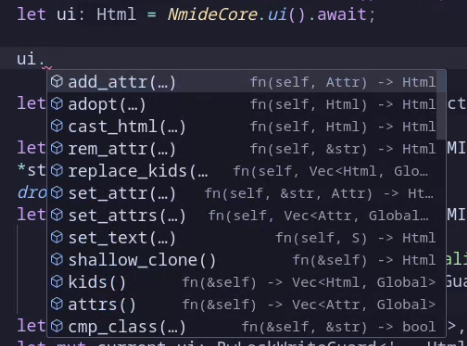
\includegraphics[width=0.5\textwidth]{context-completion.png}
  \caption{VS Code suggesting appropriate methods (Rust)}
  \label{pic:completion}
\end{figure}

\subsection{Go-to-definitions}

Being able to quickly navigate to methods and read their implementation is a
useful tool for a developer, as less time has to be spent navigating the project
structure, to figure out where some method was implemented, and more time can be
spent actually developing.

\subsection{Formatting and linting}

When developing, an important process is code review, another developer ensuring
that the suggested improvement is up to some standard, specified by the
language and/or development team. Things like naming conventions, code style,
unused variables, dangling doc-strings, bad variable names and commented out
code, have no effect on the resulting program. Unused variables and comments
are optimized away by the compiler, while variable names are mangled.\footnote{Unless they are constants}
But for developers reading the source code, these issues can hide bugs because
there is a lot of \textit{noise}. Luckily, \gls*{ide}s can detect these common
issues, by the help of a \textit{linter}, which can, on the invocation of the
user, fix these issues. Linters are opinionated, since programming language
specifications specify conventions on how the source code should look. In Rust
for example, the compiler has a built-in formatter and linter, which, during
compilation, warns the user of these mistakes, and can re-arrange the source
code by formatting it to fit the standard.

\subsection{Boilerplate code generation}

An important process in development, are ensuring your code is correct. A good
way to ensure this, is with unit testing. For object oriented programming, this
is done by testing the methods on a class, and creating the necessary unit tests
for this can be tedious. Luckily, \gls*{ide}s like IntelliJ come with
boilerplate code generation, creating a \textit{skeleton} unit test, containing
the empty tests ready to fail. An example for this can be seen in
\ref{pic:generate}, where we are prompted with a checkbox for each method on
the class; whether we want to include it in our unit test or not.

\begin{figure}
  \centering
  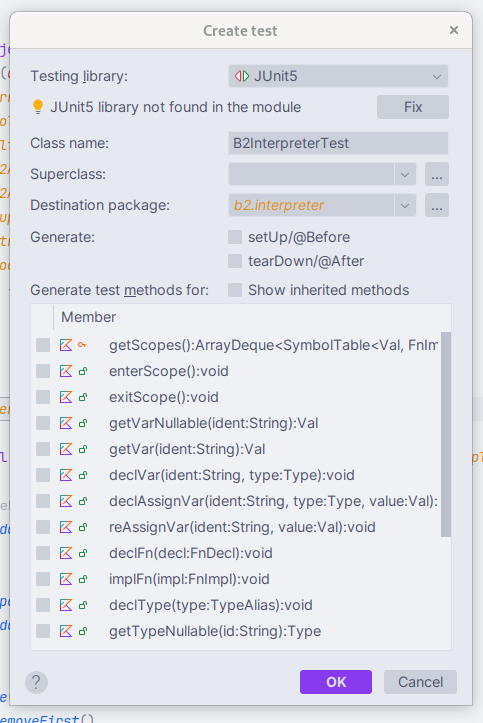
\includegraphics[height=0.5\textwidth]{generate.png}
  \caption{
    Window for generating boilerplate code for a unit test (Kotlin in
    IntelliJ)
  }
  \label{pic:generate}
\end{figure}

These are features also within a generic \gls*{ide}, but most are available
through the \gls*{ide} module architecture. A generic \gls*{ide} contains the
features that are common among development across any programming language. But
the following features are not exclusive to generic \gls*{ide}s.

\subsection{File explorer}

Most project nowadays is larger than one file, so being able to visualize the
project in a tree-like-structure, and navigate that, is useful. Similarly to
syntax highlighting, it adds icons to showcase what is a file or folder, but
also what file extension is used. In the picture \ref{pic:fileEx}, one can see
how all the Rust files, the files ending with \textit{rs}, have a crab\footnote{Called \textit{Ferris}},
visually showing the developer that this file is a Rust source file. This makes
it easier for a developer working on a polyglot project, as they can quickly
find source files by language. This feature also comes with the ability to
manipulate the project structure, by adding files, folders, moving files around,
and deleting them, but most importantly, being able to open the file. By
clicking on a file, it opens up in an editor, to be edited.

\begin{figure}
  \centering
  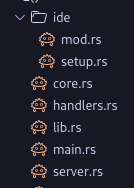
\includegraphics[width=0.25\textwidth]{file-explorer.png}
  \caption{File explorer in VS Code showing the Nmide source code}
  \label{pic:fileEx}
\end{figure}

\subsection{Version Control System integration}

Version Control System is an integral part of development. Being able to sync
ones work between different machines and developers is essential. It allows for
cooperation between different programmers.

In the picture \ref{pic:vcsViz}, we can see an example of this in action. There,
we are using Git to version control our project, (this \gls*{ide}). Vim
can detect changes made to the project, with the help of Git, adding colours to
our files based on their state, not controlled, uncommitted changes, marked
changes, committed change.

\begin{figure}
  \centering
  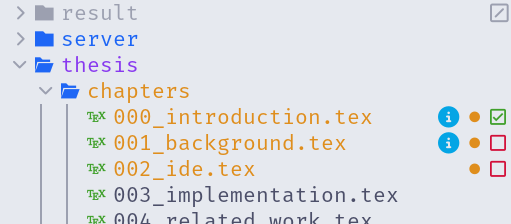
\includegraphics[width=0.5\textwidth]{vcs-viz.png}
  \caption{
    File explorer in Vim showing that the \textit{result} folder is not
    controlled by Git (grey), and that the thesis folder have uncommitted
    changes, (purple), the files who have changes are marked (yellow), and there
    is one file which has a committed, but a non-pushed change, (green checked
    checkbox).
  }
  \label{pic:vcsViz}
\end{figure}

\subsection{Module market and module installation}

An important part of the user experience in a modular \gls*{ide}, is being able
to seamlessly add, install and use modules. An integral part of this is the
module marketplace. This is a term for the place where a user can find modules,
and with the click of a button, install them. Depending on what feature this
module adds, the installation process could be as simple as adding it during the
runtime, or if it's a more complex or integrated feature to the \gls*{ide},
requires a restart of the \gls*{ide}. In the picture \ref{pic:market}, we can see
this in action.

\begin{figure}
  \centering
  
\includegraphics[width=0.5\textwidth]{module-market.png}
  \caption{
    Module market window in IntelliJ showing popular modules that the user can
    install by clicking on the \textit{install} button. Also seen in the window is
    that the user can disable already installed modules, or uninstall them.
  }
  \label{pic:market}
\end{figure}


\section{Zero-core module architecture} \label{sec:architecture}

A modular application, is an application which can be extended by other pieces
of software. This extensibility is useful as features that the original
developers of the application did not think about, can be added. If this module
architecture is well-designed, then this extension can be added without changing
the core application.

There are different ways an application can be extended. The most common one
uses so-called \textit{live-reload}, in which, if a module drastic changes the
functionality of an application, the application has to be restarted, or if it
is a \textit{minor} change, the module is simply loaded. Commonly, \gls*{ide}s
are extended during runtime. Another method would be
\textit{compile-time-extension}, in which modules are added before the
application itself is compiled. There are some advantages and disadvantage in
both approaches.

\subsection{Compile-time module}

As an example, a standard user of any application will expect the application to
come bundled with all the needed functionality. This is best achieved with the
\textit{compile-time-extension} method, since the application can be installed
with the expected modules during compile time, ensuring the resulting binary
contains all the wanted features. This also comes with the benefit of the
compiler being able to optimize the module-core interactions, since the module
is directly integrated into the source code of the core application.

\subsection{Runtime module}

Runtime modules are usually also interpreted, but they can still be a
library that is loaded during runtime. The benefit with a runtime module,
is that a user can easily test out different modules, as compiling the entire
application before being able to test a module is a hassle. But it comes with
some drawbacks, like having to do extra verifications on top of the module,
ensuring invoking the module won't crash the entire \gls*{ide}.


\subsection{Zero-core IDE}

A zero-core \gls*{ide} takes the modular architecture that is standard
\gls*{ide}s and takes it to its extreme. When all features are modules, and
modules interact by invoking each other, it can mimic a microservice
architecture. A module invocation is some \textit{request}, which the invoked
module \textit{responds} to. There is a provider-consumer dynamic. There is a
provider, some module providing data, and some consumer, some module using the
data.

If either the consumer or the provider is maintained by a third party, then
there is some informal \textit{contract} between them. The consumer expects the
outputs of a provider to be in some certain format, which in the case for
\gls*{rest} \gls*{api}s usually is \gls*{json}, and with specification formats
like OpenApi\footnote{https://swagger.io/docs specification/v3\_0/about/}, one
can also specify the structure of the \gls*{json} response, with what fields and
values it can have. One can also specify what values are valid in a request.

But even if one does use such a format, changes in scope can require the
provider to change the \gls*{api}, which could affect the consumer, because the
consumer assumed something about their informal contract, that all numbers
provided are integers. And if suddenly the provider changes, and returns
floating point numbers, the consumer could crash trying to parse a string as an
integer.

The same concept applies to a zero-core \gls*{ide}. Modules have an implicit, and
informal contract between them. So the same measures, used in microservice
architecture, to mitigate these issues, can be used in this zero-core \gls*{ide}.
Unit testing of code is essential in software development, especially when
developing against third party systems. Instead, invoking these third party
systems at test time, mocking is used. This mocking is part of how a consumer
assumes a provider should act. Mocking of modules is trivial, as all one needs
to mock is the state, the \gls*{ui}, or that some event happens, triggering a
module. At a larger scale we test the module family, to see if its change has
affected the other modules.

This can be done with contract testing, as discussed by Gross and
Mayer~\cite{GROSS200322}. They propose a component architecture, where each
module exposes some testing interface. The same principals they discussed, while
for a different, but similar architecture, can be applied to ours. But instead
of having each module have a testing interface, we can instead load all modules
composing the \gls*{ide} in a test environment, where all interactions are
recorded, and used to generate a dependency graph, showing what modules depend
on whom. This can show that certain modules are more tightly connected than
assumed, meaning they are in the same module family, it can also show what
module families communicate with other module families, showing module
communities.


\subsection{Module ecosystem}

In modern \gls*{ide}s, with an extensive module architecture, there exists a
vast module ecosystem. From simple modules that change the color scheme, or
add file icons to more complex modules that add support for other languages.
A good variety of a module ecosystem can help ensure the longevity of an
\gls*{ide}. In the table \ref{tbl:mod}, we can see that \gls*{ide}s have an
extensive module ecosystem.\footnotemark{}

\footnotetext{Data found by looking at the marketplace for the modules, in order:\url{https://marketplace.eclipse.org/content/welcome-eclipse-marketplace}, \url{https://plugins.jetbrains.com/}, \url{https://marketplace.visualstudio.com/search?target=VSCode\&category=All\%20categories\&sortBy=Installs}}

VS Code is a popular \gls*{ide}~\cite{topIde}, and this could be due to
the amount of modules it has to offer. The amount of modules attributed to
VS Code could be the cause of a positive feedback loop. VS Code is
popular because it has many modules to extend the functionality, making it able
to cover many use cases. Since VS Code is popular, developers use, and make
modules for VS Code. All of which strengthen the longevity of the
\gls*{ide}.

\begin{table}[]
  \centering
  \caption{Module Ecosystem per \gls*{ide}}
  \label{tbl:mod}
  \begin{tabular}{|l|l|}
    \hline
    \gls*{ide} & Module count \\ \hline
    Eclipse & $\sim1200$ \\ \hline
    IntelliJ & $\sim9500$ \\ \hline
    VS Code & $\sim71700$ \\ \hline
  \end{tabular}
\end{table}


\subsection{Granularity}

When designing modules, the \textit{granularity} of the combined modules has to
be considered. As an example, if one where to extend the zero-core application
with the needed functionality for it to be considered an \gls*{ide}, this could be
achieved by creating a singular module which does all the work. However, this
is not a modular approach, as if one wants to change some specific feature in
the \gls*{ide}-module, one would have to re-create the whole module with that
specific feature implemented. Instead, if this functionality was granular,
that is to say, split into several modules, that together enable the needed
features, then it would be \textit{simpler} to modify the needed modules to
achieve the wanted feature.


\subsection{Module family}

A module family are several modules enabling a single
\textit{feature}. A user of the \gls*{ide} might think that being able to browse
the project using a file explorer integrated into the \gls*{ide} as a single
feature but, in a modular system that facilitates reuse, this would be made up
of several different modules.

\begin{figure}[H]
  \centering
  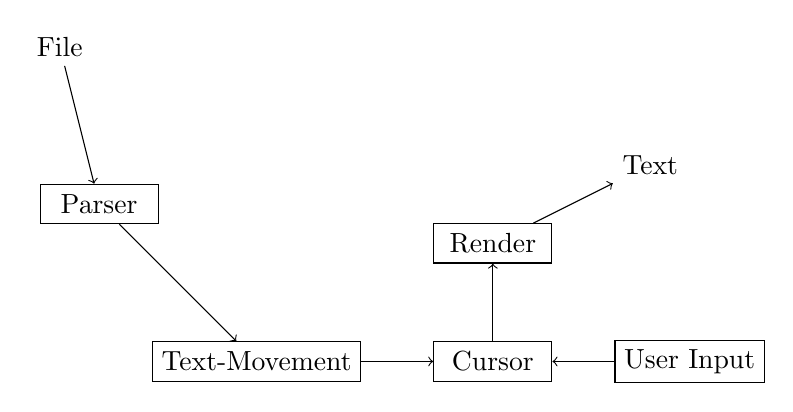
\begin{tikzpicture}
  % Nodes
  \node (file) [] at (-6, 3) {File};
  \node (parser) [rectangle, draw, minimum height=0.5cm, minimum width=1.5cm] at (-5.5, 1) {Parser};
  \node (text-movement) [rectangle, draw, minimum height=0.5cm, minimum width=1.5cm] at (-3.5, -1) {Text-Movement};
  \node (cursor) [rectangle, draw, minimum height=0.5cm, minimum width=1.5cm] at (-0.5, -1) {Cursor};
  \node (user-input) [rectangle, draw, minimum height=0.5cm, minimum width=1.5cm] at (2, -1) {User Input};
  \node (render) [rectangle, draw, minimum height=0.5cm, minimum width=1.5cm] at (-0.5, 0.5) {Render};
  \node (text) at (1.5, 1.5) {Text};
  % Arrow
  \draw[->] (file) -- (parser) node[midway, above] {};
  \draw[->] (parser) -- (text-movement) node[midway, above] {};
  \draw[<-] (cursor) -- (text-movement) node[midway, above] {};
  \draw[<-] (cursor) -- (user-input) node[midway, above] {};
  \draw[->] (cursor) -- (render) node[midway, above] {};
  \draw[->] (render) -- (text) node[midway, above] {};
\end{tikzpicture}

  \caption{Diagram of a module family for a text editor}
  \label{fig:textEditorSimple}
\end{figure}

In figure \ref{fig:textEditorSimple}, an input file is parsed to some structure
which is used to translate user actions, into cursor movements. The cursor being
the place in the file where text is written to by the user.

Module families naturally shows up in a \textit{true} modular system. If
several modules together enable some feature, then those modules can be treated
as a singular module by an external module developer, depending on what they
want to extend.


\subsection{Existing Magnolia IDE}

The current \gls*{ide} for Magnolia~\cite{baggeIde}, is a many-years-old version
of Eclipse, using modules and functionality from the core Eclipse application,
that has since been outdated. The \gls*{ide}s lifetime was limited by a
dependency on external modules and features that where not maintained by the
\gls*{ide}-developers. This meant that for future development of Magnolia, an
outdated \gls*{ide} was needed, with outdated tooling. Furthermore, the Magnolia
compiler was implemented as an Eclipse module, which means that development is
limited to Eclipse, and only Eclipse, as a developer cannot compile Magnolia
code without it.

Modularization will help to mitigate some of the issues with the current
Magnolia \gls*{ide}. Instead of maintaining an entire application, the needed and
wanted features of the application can be maintained instead.

Experimental languages might have features which are not possible to be fully
used in current \gls*{ide}s. This is also the case for the current Magnolia
\gls*{ide}. The compiler for Magnolia, syntax highlighting, error reporting, and
hover-functionality are functionality made in the Eclipse \gls*{ide}, by using
its plug-in architecture. Some of the functionality and plug-ins this
implementation used, have been deprecated in later version of Eclipse. This
means the Magnolia \gls*{ide} is locked to an old version of Eclipse, which, as
time passes, increases the complexity of installation, as the surrounding
tooling and libraries needed by this version of Eclipse also becomes deprecated.
Currently, in INF220, a course at the university, two weeks are set aside for
students to be able to install the current Magnolia \gls*{ide}.


\section{Challenges imposed by Magnolia} \label{sec:challenges}

In most programming languages, any type has a singular definition, retrieving
the file and position in the file, where a type is implemented, is trivial, as
there is only one position to show or go to. However, in Magnolia a singular
type could have multiple definitions, and resolving this can be complex.
Especially communicating this to a user in a helpful manner.


\subsection{Renaming}

Given our definition of a monoid\footnotemark[12]{}, one can trivially see that
string concatenation and list concatenation falls under this definition, and are
therefore related. It is therefore quite reasonable to reuse the monoid
concept, within the string and list concepts. Along side their respective
methods, like \textbf{toUpperCase} or \textbf{map}.

Even though they are related, it is more useful to have specific names for each
concept. In \ref{lst:strConc} and \ref{lst:lstConc} we are importing the
monoid\footnotemark{}, and renaming the \textbf{unit} and \textbf{binop}
operation to something that are specific to the concepts, \textbf{emptyString},
$+$ and \textbf{emptyList}, $++$ respectively.

\footnotetext{Definition \ref{def:monoid}}

\begin{code}[H]
  \lstinputlisting
    [ language=Magnolia
    , caption={String concatenation (Magnolia)}
    , label=lst:strConc
    ]{./code/string-conc.mg}
\end{code}

\begin{code}[H]
  \lstinputlisting
    [ language=Magnolia
    , caption={String concatenation (Magnolia)}
    , label=lst:lstConc
    ]{./code/list-conc.mg}
\end{code}

In Magnolia, it is useful for a developer to visualize and follow the effect of
renaming, that the compiler does. This visualization would enable a developer
to know where a renaming happens. The structure of this is tree-like. It is
quite useful to visualize tree-like structures, and such functionality is not
typically something an \gls*{ide} offers. It would be helpful, then, if the new
Magnolia \gls*{ide} can visualize different structures. Such features should be
implemented using modules.

\subsection{Dependency cycles}

A cyclic dependency, is an issue in programming, where different libraries
depend on each other, and the compiler or interpreter cannot easily find out
which library to compile/interpret first. In the figure \ref{fig:depIssue}, we
can see a visualization of such a dependency issue.

\begin{figure}[H]
  \centering
  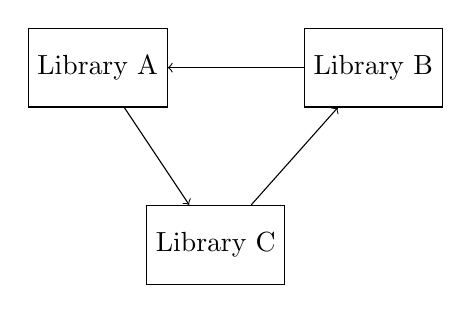
\begin{tikzpicture}
  \node (tool) [rectangle, draw, minimum height=1cm, minimum width=1cm] at (2.5, -0.75) {Library A};
  \node (ide) [rectangle, draw, minimum height=1cm, minimum width=1cm] at (6, -0.75) {Library B};
  \node (module-reg) [rectangle, draw, minimum height=1cm, minimum width=1cm] at (4, -3) {Library C};

  \draw[->] (tool) to node[midway, above] {} (module-reg);
  \draw[->] (ide) to node[midway, above] {} (tool);
  \draw[->] (module-reg) to node[midway, above] {} (ide);
\end{tikzpicture}

  \caption{
    Diagram of a cyclic dependency. Library A depends on library B, which
    depends on library C, which depends on library A, it is not clear in which
    order to parse the library.
  }
  \label{fig:depIssue}
\end{figure}

Library A, creates some functionality, that library B needs, in its own
functionality. Finally, library C uses functionality from library B, which
library A depends on, creating a cycle.

Programming languages have different ways to avoid the problem of imports of
modules forming a cyclic graph. The easiest, is to simply disallow such import
structures, which is something the Magnolia compiler does. All imports have to be
\gls*{dag}'s.

In most programming languages this is trivial to solve for developers, as if
suddenly a project has a cyclic import, it can be solved quite easily. However,
due to the heavy reuse in Magnolia, the cycles could be quite large and harder
to reason about without a tool to visualize the dependency graph.


\subsection{External software dependency}

Magnolia depends on a compiler, like all compiled programming languages, but
also an \gls*{smt} solver. While the new compiler for Magnolia, at the time of
writing is still under development~\cite{wiig}, but once released will be quite
stable. Writing modules that utilize the new compiler can be tightly coupled
with the compiler.

This is in contrast to the \gls*{smt} solver environment. Skogvik~\cite{beateVerification}
noted the different competitions for developers of \gls*{smt} solvers, this
means there might be a new and better \gls*{smt} solver, which means it needs to
be easy for a user of the \gls*{ide} to change the \gls*{smt} solver they are
using to validate their program with. Since due to such \gls*{smt} solver
competitions, newer versions and solvers are created, and should be usable in a
modular \gls*{ide}.
